\documentclass[TS,lsstdraft,toc,usenatbib]{lsstdoc}

% Package imports go here
\usepackage{amsmath}	% Advanced maths commands
\usepackage{amssymb}
\usepackage{gensymb}  % degree symbol 
\usepackage{natbib}  % bibliography
\usepackage{cprotect} 
% Local commands go here

%% Journal abbreviations
%\bibliographystyle{aasjournal}

\title[Dome crawling implementation]{Dome crawling implementation on LSST Scheduler Observatory Model} 

\author{Tiago Ribeiro} 

\setDocRef{Document-XXX}
\date{\today}
\setDocRevision{v0.1}
\setDocStatus{draft}
\setDocAbstract{%
Description of the implementation of dome crawling in the LSST Scheduler Observatory Model
}

% Change history defined here. Will be inserted into
% correct place with \maketitle
% OLDEST FIRST: VERSION, DATE, DESCRIPTION, OWNER NAME
\setDocChangeRecord{%
\addtohist{1}{2018-05-16}{First released version.}{Tiago Ribeiro}
}

\begin{document}

% Create the title page
% Table of contents will be added automatically if "toc" class option
% is used.
\maketitle


\section{Introduction} 
\label{sec:intro}

% It provides means to estimate the time required for going from one state to another, as well as determining if a state transition is possible or not. 

The LSST Observatory Model is a key component of the LSST Scheduler. The observatory model keeps track not only of the absolute position (altitude, azimuth, camera rotation angle, etc) of the telescope and dome but also the housed filters and so one. 

The main functionality of the Observatory Model is to estimate the slew time required between an initial and final state of the observatory. Currently, this state transition accounts for changes in the main observatory components, including; 
%
\begin{enumerate}
\item Telescope altitude, with maximum and minimum limits. Since LSST is an AltAz telescope it cannot track objects close to zenith, so a limit on the maximum altitude is important for precise modeling of the telescope behavior. 
\item Telescope azimuth, with cable wrap limits. 
\item Camera rotation angles, with cable wrap limits. 
\item Dome altitude and azimuth. It is important to note that the LSST dome must be positioned in both altitude and azimuth. This is a requirement on the system design to mitigate wind-induced vibrations as well as stray light contaminations. Also, the dome does not have any azimuth wrap limits. 
\item Filter change. 
\item Optics open loop.
\item Optics closed loop.
\end{enumerate}
%
For telescope, dome and camera rotation, a second-order kinematic model, that accounts for constant acceleration/deceleration, maximum speed and limits is used.

The model works in an hierarchical way, meaning that each "slew activity" contains a list of "prerequisites". An activity cannot start until its prerequisites are completed. As such, activities that does not depend on the others can happen in parallel, and the model assumes only the longest one. For instance, telescope altitude and azimuth motion happens in parallel with each other and also with dome altitude and azimuth, and only the longest activity will actually contribute to the total slew time.

To compute the time required for a slew activity to complete, the model first computes the travel distance, properly handling those axis that have wrap limits. This means, if an axis is at absolute position $260^\circ$  and a final position angle of $280^\circ$   is requested for an axis that has a wrap limit of $270^\circ$, the total travel distance is going to be $340^\circ$ instead of $20^\circ$ and the final absolute position is $-80^\circ$.

A key aspect of the LSST system is that the telescope is extremely fast to slew from one position to another. The baseline parameters for the telescope kinematic models are, an acceleration/deceleration of $3.5^\circ/s^2$ and max speed of $3.5^\circ/s$. At the same time, the dome is not as fast as the telescope, with an acceleration of $0.75^\circ/s^2$ and max speed of $1.5^\circ/s$, in the azimuth direction. 

In order to mitigate that issues, the real system is designed to have a slightly oversized dome on the azimuth direction, that would enable two neighboring fields to be visited without the need to slew the dome. That, combined with a so called "dome crawling mode" make it possible to eliminate, or at least mitigate, the speed diference between the dome and the telescope. So far, the observatory model did not considered this crawling mode (or the oversize of the dome in azimuth) on the computations, which could severely impact the results of the simulations. In fact, recent simulations done with dome crawling shows an increase of up to 3\% on the total number of visits over the course of the 10 years of the survey. 

The implementation of dome crawling (and the oversized slit effect) was done on the observatory kinematic model by adding a new parameter called "free range". Basically, this parameter specifies how far ahead you can slew before the slew actually starts. For instance, if the "free range" is $4^\circ$, then any slew equals to or smaller than that will just have a delay of zero seconds. If the slew is longer than that, the model computes the speed achieve by accelerating at maximum rate for that distance and what speed you have to be at the end so it is possible to decelerate to stop in that same distance. The total travel distance, is the difference between the original travel distance and the free range. So, overall, what the free range parameter does is to decrease the travel distance and enables the system to travel at a higher average speed. Another important consideration is that dome crawling has no settling time. On the regular dome setup models, the settling time is, in principle, used to synchronize the dome and the telescope position to millimeter precision, in order to avoid vignetting of the FoV. For an oversized dome slit it is actually not necessary to align both to that precision. 

Finally, one key aspect of the actual operation of dome crawling is that the control software needs to know where the system is going to point ahead of time, so it can actually prepare accordingly. For the model, we just assume that this is known in advance when computing the slew time. Since the LSST Scheduler is required to publish the next visit with a lead time, this probably won't be a problem for operating the dome in this mode. 

\subsection{Results}

Figure~\ref{fig:comparison} shows a comparison of slew times (a.k.a. delay) against total travel distance for the kinematic model using the default values for dome azimuth with a free range of $0^\circ$ (no dome crawling) and $4^\circ$ (crawling considering the designed oversize of the dome slit compared to the FoV). 

\begin{figure}[htbp]
\begin{center}
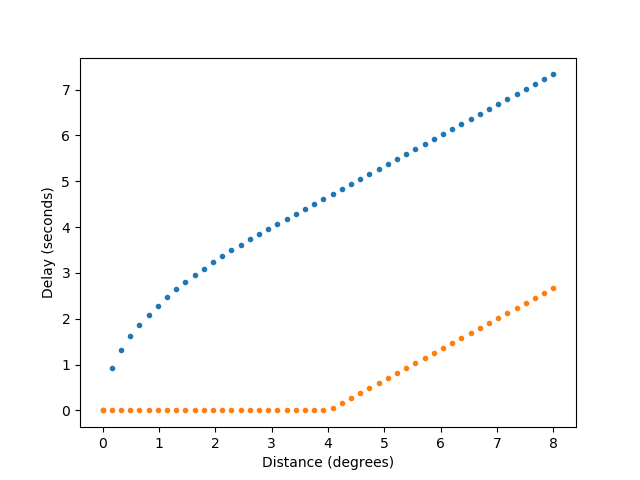
\includegraphics[width=0.8\columnwidth]{images/figure_1}
\caption{default}
\label{fig:comparison}
\end{center}
\end{figure}

As explained on Section~\ref{sec:intro}, the delay is zero for travel distances lower than or equal to the free range. At the same time, the default kinematic model with settling time has a floor value of $1 \rm s$, the settling time. Also note growth curve of the delay for the non-crawling kinematic curve. It starts with a quadratic behavior until it reaches the maximum speed, then transitioning to a linear behavior, after about 2 seconds. At the same time, when "crawling", the delay time starts at the linear behavior, which means it is already at maximum speed for this particular configuration. 




\end{document} 



